                 %% ****** Start of file template.aps ****** %
%%
%%
%%   This file is part of the APS files in the REVTeX 4 distribution.%!TEX encoding = UTF-8 Unicode
%%   Version 4.0 of REVTeX, August 2001
%%
%%
%%   Copyright (c) 2001 The American Physical Society.
%%
%%   See the REVTeX 4 README file for restrictions and more information.
%%
%
% This is a template for producing manuscripts for use with REVTEX 4.0
% Copy this file to another name and then work on that file.
% That way, you always have this original template file to use.
%
% Group addresses by affiliation; use superscriptaddress for long
% author lists, or if there are many overlapping affiliations.
% For Phys. Rev. appearance, change preprint to twocolumn.
% Choose pra, prb, prc, prd, pre, prl, prstab, or rmp for journal
%  Add 'draft' option to mark overfull boxes with black boxes
%  Add 'showpacs' option to make PACS codes appear
%  Add 'showkeys' option to make keywords appear
%\documentclass[aps,prstab,twocolumn,superscriptaddress,showpacs]{revtex4}


\documentclass[aps,prstab,superscriptaddress,showpacs]{revtex4-1}

%
% NEED THIS FOR THE TODO's
%
%\textwidth  15cm
%\marginparwidth 2cm
%
% ------------------------------------------
%
\usepackage{amsmath}
\usepackage{graphicx}
\usepackage{subfigure}
\usepackage{url}
\usepackage[colorlinks,linkcolor=blue,anchorcolor=blue,citecolor=blue]{hyperref} % hyper reference to contents
\usepackage{algorithm,algorithmic}
\usepackage{tikz}
\usepackage{suffix}
\usetikzlibrary{arrows,shapes,snakes}
\bibliographystyle{apsrev4-1}

\newcommand{\opal}{\textsc{OPAL}}
\newcommand{\opalt}{\textsc{OPAL-t }}
\newcommand{\opale}{\textsc{OPAL-e }}
\newcommand{\opalcycl}{\textsc{OPAL-cycl}}
\newcommand{\opalmap}{\textsc{OPAL-map }}
\newcommand{\opalenv}{\textsc{OPAL-envelop}}

\newcommand{\mad}{\textsc{mad }}
\newcommand{\madnine}{\textsc{mad9 }}
\newcommand{\madninep}{\textsc{mad9p }}
\newcommand{\madeight}{\textsc{mad8 }}

\newcommand{\classic}{\textsc{classic }}
\newcommand{\hfifepart}{\textsc{H5Part }}
\newcommand{\hfifefe}{\textsc{H5FED }}

\renewcommand{\epsilon}{\varepsilon} 
\renewcommand{\vec}[1]{{\bf #1}} 
\newcommand{\dt}[1]{\frac{\partial #1}{\partial t}}
\newcommand{\dtt}[1]{\frac{\partial^2 #1}{\partial t^2}}
\newcommand{\dtvec}[1]{\frac{\partial {\mathbf #1}}{\partial t}}
\newcommand{\dttvec}[1]{\frac{\partial^2 {\mathbf #1}}{\partial t^2}}
\newcommand{\rot}{\vec{\nabla} \wedge }
\renewcommand{\div}{\vec{\nabla} \cdot }

\def\vec#1{\mathbf{#1}}
\def\vecg#1{\boldsymbol{#1}}
\def\norm#1{\| #1 \|} 
\def\tr{^{\!\top}}

\def\curl{{\bf curl}\,}
\def\curlp{{\rm curl}_p\,}
\def\div{{\rm div}\,}
\def\grad{\nabla}
\def\gradp{\nabla_p}
\def\dotp#1#2{\langle#1,#2\rangle}
\def\eps{\varepsilon}

\newcommand{\mat}[1]{\ensuremath{\boldsymbol{#1}}}
\newcommand{\vect}[1]{\ensuremath{\mathbf{#1}}}
\newcommand{\iprod}[2]{\ensuremath{\langle#1,#2\rangle}}
\newcommand{\abs}[1]{\ensuremath{|#1|}}

\newcommand{\Nedelec}{N\'{e}d\'{e}lec}

\newcommand{\id}[1]{\structure{#1}}

\newcommand {\Co}{{\mathbb{C}}}
\newcommand {\Int}{{\mathbb{Z}}}
\newcommand {\Nat}{{\mathbb{N}}}
%
%
\newcommand {\Hcurl}{{H(\mathbf{curl};\Omega)}}
\newcommand {\Hocurl}{{H_0(\mathbf{curl};\Omega)}}
\newcommand {\Hdiv}{{H(\mathrm{div};\Omega)}}
\newcommand {\Hodiv}{{H_0(\mathbf{div};\Omega)}}
%
\renewcommand {\Re}{{\rm I \kern-2pt R}}
\newcommand{\vc}[1]{\mbox{\boldmath $#1$}}
\newcommand {\RM}[1]{\mathrm{#1}}



% A simple colored box inlined with the text
%  #1: color to use
%  #2: text to put
\newcommand{\INLINEBOX}[2]{%
   \begin{center}%
    \fcolorbox{#1!60!black}{#1}{%
      \addtolength{\linewidth}{-0.6cm}%  fixed value, works for normal article text
            \begin{minipage}{2\linewidth} #2 \end{minipage}%
  \begin{minipage}{\linewidth} #2 \end{minipage}%
    }%
   \end{center}\vspace{1pt}%
}

% A box at the margin containing the given text
\newcommand{\MARGINBOX}[1]{%
  \mbox{}%
  \marginpar%
   [\tiny\raggedleft\hspace{0pt}#1]%
   {\tiny\raggedright\hspace{0pt}#1}%
}

% mark specific elements: starred versions use inline boxes
\newcommand{\TODO}[2][]{\MARGINBOX{\textcolor{red!80!black}{\emph{ToDo (#1):}} #2}}
\WithSuffix\newcommand\TODO*[2][]{\INLINEBOX{red!20!white}{\emph{ToDo (#1):} #2}}

\newcommand{\FIXME}[2][]{\MARGINBOX{\textcolor{blue!80!black}{\emph{FixMe (#1):}} #2}}
\WithSuffix\newcommand\FIXME*[2][]{\INLINEBOX{blue!20!white}{\emph{FixMe (#1):} #2}}

\newcommand{\NOTE}[2][]{\MARGINBOX{\textcolor{green!80!black}{\emph{Note (#1):}} #2}}
\WithSuffix\newcommand\NOTE*[2][]{\INLINEBOX{green!20!white}{\emph{Note (#1):} #2}}

\newcommand{\DRAFT}[2][]{\MARGINBOX{\textcolor{blue!80!black}{\textsc{Draft (#1):}} #2}}
\WithSuffix\newcommand\DRAFT*[2][]{\INLINEBOX{blue!20!white}{\textsc{Draft (#1):} #2}}


\newcommand{\bs}[1]{\mathbf #1}
\renewcommand{\baselinestretch}{2.0}

\begin{document}
\tikzstyle{format} = [draw, thin, fill=blue!20]
\tikzstyle{pblock} = [rectangle, draw, fill=blue!20, text width=12em,text centered, rounded corners, minimum height=0.4em]
\tikzstyle{pblockll} = [rectangle, draw, fill=blue!20, text width=25em, text centered, rounded corners, minimum height=0.4em]
\tikzstyle{pblockl} = [rectangle, draw, fill=blue!20, text width=11.5em, text centered, rounded corners, minimum height=0.4em]
\tikzstyle{pblocks} = [rectangle, draw, fill=blue!20, text width=8em, text centered, rounded corners, minimum height=0.4em]
\tikzstyle{decision} = [diamond, draw, fill=blue!20, text width=5em, text badly centered, node distance=3cm, inner sep=0pt]
\tikzstyle{medium} = [ellipse, draw, thin, fill=green!20, minimum height=2.5em]
\tikzstyle{cloud} = [draw, ellipse,fill=red!20, node distance=3cm, minimum height=2em]
\tikzstyle{line} = [draw, -latex']
\tikzstyle{emptyblock} = [rectangle]
\tikzstyle{progblock} = [rectangle, draw, fill=yellow!20, text width=6em, text centered, minimum height=0.4em]
\tikzstyle{null} = [rectangle, fill=blue!0, text width=0em, text centered, rounded corners, minimum height=0.4em]
\tikzstyle{cpoint} = [draw,circle,fill=white,minimum size=1pt,
                            inner sep=0pt]
\tikzstyle{cblock} = [circle, draw, fill=blue!20, text width=3m, text centered, rounded corners, minimum height=0.4em]

\graphicspath{figures}

\title{On Dark Current and Multipacting Simulation Capabilities of \opal\\ - Modeling, Benchmarking and Applications} %\\ submitted to Phys. Rev. STAB

\author{Ch. Wang}
\email{cwang@ciae.ac.cn}
\affiliation{China Institute of Atomic Energy, Beijing, 102413, China}
\affiliation{Paul Scherrer Institut, Villigen, CH-5232, Switzerland}
\author{A. Adelmann}
\email{andreas.adelmann@psi.ch}
\affiliation{Paul Scherrer Institut, Villigen, CH-5232, Switzerland}
\author{M. Seidel}
\affiliation{Paul Scherrer Institut, Villigen, CH-5232, Switzerland}
\author{Y. Ineichen}
\affiliation{Paul Scherrer Institut, Villigen, CH-5232, Switzerland}
\author{T. J. Zhang}
\affiliation{China Institute of Atomic Energy, Beijing, 102413, China}
\noaffiliation

\begin{abstract}
Dark current and multiple electron impacting (multipacting), as observed in radio frequency (RF) structures of accelerators, 
are usually harmful to the equipment and the beam quality.
These effects need to be suppressed to guarantee stable operation. Large scale
simulations can be used to understand the cause and develop solutions for these
phenomena.
 
We extend \opal\, a parallel framework for charged particle
optics in accelerator structures and beam lines, with the necessary physics models
to simulate these phenomena. This is achieved by adding a Fowler-Nordheim
field emission model and two secondary electron emission models, developed by Furman-Pivi and Vaughan respectively, as well as efficient 3D boundary geometry handling capabilities to \opal.

In situations where the electron multiplication is severe, we have to re-normalize the simulation particles in order to prevent excessive memory consumption. 

A carefully benchmark against a non-stationary multipacting theory for the classic parallel plate geometry will be presented.

Preliminary results on dark current simulations of the CTF3 electron source and first multipacting simulation in large RF cavities for compact high intensity cyclotrons will be presented.

\end{abstract}

\pacs{29.20.dg;29.27.Bd;41.85.Ew}

\maketitle

\section{INTRODUCTION \label{intro}}
Dark current and multipacting phenomena have been observed in various RF structures of accelerators. The dark current in electron guns, which is generated by field emission due to the strong accelerating field in the gun cavity \cite{J-H-Han} and multipacting appearing in high-Q RF cavities of cyclotrons \cite{CY, riken}, are two well known examples. These phenomena are usually harmful to the equipment and beam quality, as they will cause galvanic etching on the surface of the cavity and thus cause RF breakdown.

The dark current in the electron gun of a FEL facility may make severe hazards, radiational activation and even mechanical damage to diagnostic systems and undulator sections \cite{J-H-Han}. 

And the multipacting in cyclotron cavities is a very disturbing phenomenon. The seed electrons will impact the cavity surface, produce new electrons. Under certain conditions (material and geometry of the RF structure, frequency and level of the electromagnetic field, with or without the appearance of the magnetic field \ldots), electrons secondary emission yield (SEY) coefficient will be larger than one and lead to exponential multiplication of electrons. This kind of discharge will limit the power level until the surfaces will be cleaned through a conditioning process. But this process is very time-consuming. \cite{CY, riken}

 Large scale dark current and multipacting simulations based on reliable data of surface material, full size geometry model of RF structures and parallel computing allow more thorough analysis and a deeper understanding of these phenomena even in early design stage of RF structures.  

To make \opal\ \cite{opal:1} a feasible tool to perform large scale dark current and multipacting simulations, first we implement a 3D particle-boundary collision test model into \opal\ to facilitate the particle searching during tracking process. In a subsequent step we add surface physics models including an analytic Fowler-Nordheim field emission model and two secondary emission models, developed by Furman-Pivi and Vaughan respectively, into \opal.

The above mentioned models and their implementation in \opal\ have been benchmarked against a non-stationary theory \cite{Non} with a parallel plate geometry. The time evolution of particle number agrees very well.

% Here the intro to application

\section{BASIC EQUATIONS AND PHYSICAL MODELS }


\subsection{Geometry Handling}
Testing particle-boundary collisions is crucial to both dark current and multipacting simulations. Since complex 3D geometries are hard to be accurately parametrized by simple functions, we use triangulated surfaces, which are extracted from volume mesh generated either by GMSH \cite{gmsh} or Heronion \cite{heronion}, to represent the complex geometry of real RF structures. Subsequently we can make use of efficient 3D line segment-triangle intersection (LSTI) tests to find particle-boundary collisions. 

The algorithm of the LSTI test we use is from Ref~\onlinecite{LT}, and detailed introduction on our implementation can be found in our previous paper \cite{WangHB2010:1}. Even though the implemented LSTI algorithm use precomputed triangle normals which can be reused by further early rejection strategy and thus is cheaper than other algorithms \cite{LT}, a huge number of LSTI calls in each simulation time steps are necessary. If we have $M$ triangles and $N$ particles in the simulation, both in the magnitude of hundreds of thousand to millions, the number of LSTI tests in single time step without a early rejection strategy would be $M \times N$, i.e., at least $10^{10}$ per time step. Obviously, effective early rejection strategies (see Figure~\ref{fig:P-B}) are needed to reduce the number of LSTI tests.  

\begin{figure}[H]
    \begin{center}
        /Users/adelmann/svnwork/adelmann/papers/figures/Latex-Figures/2d_grid.tikz
    \end{center}
    \caption{Schematic view of particle-boundary early rejection strategy. The dark
    black line represents the boundary surface, particles are colored dots with an
    attached momenta arrow and inward normals gray arrows.\label{fig:P-B}}
\end{figure}
Assuming we need to determine whether a particle with position $\mathbf{r}$
and momenta $\mathbf{p}$ hits the boundary within time step $\Delta{t}$ we apply
the following early rejection strategies:
\begin{itemize}
    \item Test if the particle is near the boundary by checking if $\mathbf{r}$
    is inside the boundary bounding boxes (illustrated by gray grids in
    Figure ~\ref{fig:P-B}). 
    \item If $\mathbf{r}$ is not in a bounding box (green particle in Figure
    ~\ref{fig:P-B}), the particle is enough far away from boundary and
    can be integrated directly.
    \item If $\mathbf{r}$ is in a bounding box (yellow particle and red particle
    in Figure ~\ref{fig:P-B}), then we check all triangles in the bounding box
    (of the corresponding particle) as well as triangles in the adjacent 26
    bounding boxes to see if the momenta of the particle has a opposite
    direction with those triangles' normals.
    \item If the momenta and triangle normal are not opposite for all triangles
    checked (the yellow particle) do particle integration.
    \item If they are opposite (red particle) check if the particle has an
    intersection with the triangles by performing the LSTI test for each
    triangle. If an intersection exists the particle will hit the boundary
    during the current time step.
\end{itemize}

Two things need to be addressed here. First the inward normal of surface triangles which point to the inner side of the geometry could be obtained by using the following algorithm. We find a point close to a triangle with a specified ID (e.g. 0) and determine if the point is inside or outside the geometry. This can be achieved by doing a ray-boundary intersection test and counting the number of intersections. Using this point we can get the orientation (inward normal) of the triangle with ID 0. Now we can get the inward normal of all surface triangles by recursively aligning the orientation of adjacent triangles of triangles whose inward normals have already been computed.

Secondly the success of the above particle-boundary collision test relies on the
fact that the distance a particles travel in one time step cannot be larger than
the bounding box size. Choosing an appropriated bounding box size ensures that a
particle will never jump over a bounding box in one time step.
\subsection{Surface physics models} 
Electron field emission is a major source of both dark current particles and primary
incident particles in secondary emission. The Fowler-Nordheim (F-N) formula
we use here to predict the emitted current density is given in (\ref{eq:units})
\cite{FN, Feng}
%
\begin{equation}\label{eq:units}
    J(\mathbf{r},t) = \frac{A(\beta E)^2}{\varphi t(y)^2}
                      \exp{\left(\frac{-B v(y)\varphi^{3/2}}{\beta E}\right)}
                      \left[\hbox{A/$m^2$}\right]
\end{equation}
%
where $J(\mathbf{r},t)$ stands for emitted electric current density in position
$\mathbf{r}$ and time $t$. The Greek letters $\varphi$ and $\beta$ denote the
work function of the surface material and the local field enhancement factor
respectively. The parameter $E$ is the electric field in the normal direction
of surface. The parameters $A$ and $B$ are empirical constants. The functions
$v(y)$ and $t(y)$ representing the image charge effects \cite{Feng} as a function
of the Fowler-Nordheim parameter $y$ with the following definition \cite{J-H-Han}
%
\begin{equation}\label{eq:imagecharge}
    y = \sqrt{\frac{e^3}{4\pi\varepsilon}}\frac{\sqrt{\beta E}}{\varphi} 
      = 3.795\times10^{-5}\frac{\sqrt{\beta E}}{\varphi} \text{.}
\end{equation}
%
In our model, we have chosen a simpler approximation originated by J. H. Han \cite{J-H-Han}
\begin{eqnarray*}
v(y) &=& a-by^2 \\
t(y) &\approx& 1 \text{.}
\end{eqnarray*}
These approximations are valid for a large range of $y$, corresponding to
typical applied electric field ranges in RF guns.

Whenever the normal components of an electric field are strong enough the field
emission current density will be limited by space charge effect \cite{Feng}. 
To cover this situation we incorporated the 1D Child-Langmuir law
%
\begin{align}\label{eq:SpaceCharge}
    J(\mathbf{r},t) & =\frac{4\varepsilon_0}{9}\sqrt{2\frac{e}{m}}\left(\frac{V^{3/2}}{d^2}\right)\notag\\
    &
    =\frac{4\varepsilon_0}{9}\sqrt{2\frac{e}{m}}\left(\frac{E^{3/2}}{d^{1/2}}\right)
    \left[\hbox{A/$m^2$}\right]
\end{align}
%
into our field emission model. $J(\mathbf{r},t)$ denotes space charge limited emission 
current density in position $\mathbf{r}$ and time $t$, $\varepsilon_0$ the
permittivity in vacuum, $E$ the normal component of electric field on the surface
and $d$ the distance from the position where $E$ is evaluated. Currently we 
choose $d$ to be equal to the distance traveled by emitted particles in one
time step, i.e., $d=\frac{\displaystyle eE\Delta{t}^2}{\displaystyle 2m_0}$ where $\Delta{t}$ is simulation
time step.

We have implemented two secondary emission models. The first one is a
phenomenological model developed by M. A. Furman and M. Pivi \cite{Furman-Pivi}. This
choice was based on the self-consistency property this particular secondary
model offers. In this context self-consistency means that if we define one incident
electron and the followed secondary emission procedure as an event, the event
generator is constructed so that
%
\begin{itemize}
    \item when averaging over an infinite number of secondary-emission events, 
    the reconstructed secondary emission yield $\delta$ and its energy spectrum
    $ d\delta/dE$ are guaranteed to agree with the corresponding input quantities 
    \item the energy integral of $d\delta/dE$ is guaranteed to equal $\delta$
    \item the energy of any given emitted electron is guaranteed not to exceed the 
    primary energy
    \item the aggregated energy of the electrons emitted in any multi-electron event 
    is also guaranteed not to exceed the primary energy.
\end{itemize}
The Furman and Pivi's secondary emission model calculates the number of secondary electrons that result from an incident electron of a given energy on a material at a given angle (see Figure~\ref{incident electrons}). For each of the generated secondary electrons the associated process: {\em true secondary}, {\em rediffused} or {\em backscattered} is recorded, as is sketched in Figure~\ref{incident electrons}.  

\begin{figure}
    \centering
    \input{figures/HB_Fig4.tikz}
    % \includegraphics[width=3 in]{incident_diagram.pdf}
    \caption{Sketch map of the secondary emission process.}
    \label{incident electrons}
\end{figure}

The other secondary emission model we use is based on a secondary emission yield formula developed by Vaughan \cite{Vaughan, VaughanRv, FS}:
\begin{subequations}
\label{Vaughanall}
\begin{eqnarray}
\delta(E,\theta)&=&\delta_0,\ \text{for}\ v \le 0 \label{eq:VaughanA} 
\\
    \delta(E,\theta)&=&\delta_{max}(\theta)\cdot (v e^{1-v})^k,\ \text{for}\ v \le 3.6 \label{eq:VaughanB} 
\\
\delta(E,\theta)&=&\delta_{max}(\theta)\cdot 1.125/v^{0.35},\ \text{for}\ v > 3.6 \label{eq:VaughanC} 
\end{eqnarray}
\end{subequations}
where 
\begin{eqnarray*}
v=\frac{\displaystyle E-E_0}{\displaystyle E_{max}(\theta)-E_0},
\end{eqnarray*}
\begin{eqnarray*}
k=0.56,\ \ \text{for}\ v<1,
\end{eqnarray*}
\begin{eqnarray*}
k=0.25,\ \ \text{for}\ 1<v\le{3.6},
\end{eqnarray*}
\begin{eqnarray*}
\delta_{max}(\theta)=\delta_{max}(0)\cdot (1+k_{\theta}\theta^2/2\pi),
\end{eqnarray*}
\begin{eqnarray*}
E_{max}(\theta)=E_{max}(0)\cdot (1+k_E\theta^2/2\pi).
\end{eqnarray*}
The secondary emission yield value for an impacting electron energy $E$ and incident angle $\theta$ w.r.t the surface normal is denoted as $\delta(E,\theta)$. Parameter $k_{\theta}$ and $k_E$ denotes the dependence on surface roughness. Both
should be assigned a default value of 1.0, which appears appropriate for typical dull surfaces in a working tube environment, and lower values down to zero or higher values, up to about 2.0, are only valid for specified cases \cite{Vaughan}. $E_{max}(0)$ is the impacting energy when incident angle is zero and secondary yield reaches its maximum value. $E_0$ is an adjustable parameter to make the first crossover energy at which the secondary yield equals to 1 be fitted to the experiment data \cite{FS}.
 
\subsection{Implementation within \opal\ and Parallel Computing} 
The above models are implemented in the object-oriented parallel PIC code
\opalt. \opalt\ is one of the flavors of the \opal\ (Object-Oriented Parallel Accelerator Library) framework \cite{opal:1}. This framework is a powerful tool for charged-particle optics in general accelerator structures and beam lines using the MAD languages with extensions. \opal\ is based on the \classic\ \cite{Classic:1} library and the $IP^2L$ framework \cite{ippl:1}. The \classic\ library is a C++ class library which provides services for building portable accelerator models and algorithms and inputting language to specify complicated accelerator systems in general. $IP^2L$ is an object-oriented C++ class library which provides abstractions for particles and structured field calculation in a data-parallel programming style. It provides an integrated, layered system of objects. The upper layers contain global data objects of physical/mathematical quantities, such as particles, fields, random numbers, and matrices of meshes and typical methods performed on these objects such as differential operators and multidimensional FFT’s. The lower layers contain the objects relevant to parallelization such as data distribution, domain decomposition, communication among processors, load balancing, and expression templates. Statistical data, such as particle position, momentum and particle type (primary bunch, field emitted electrons or secondaries), are stored in the \hfifepart\ \cite{H5part:1} file format. In a post processing step, the data can be converted into legacy VTK formatted files \cite{vtk:1} and visualized by visualization tool Paraview \cite{paraview}.

Users can customize their own dark current and multipacting simulations by specifying the value of the parameters in above models in input file. The format of input file and examples can be found in \opal\ user guide \cite{opal:1}.

Motivated by the fact that the population of particles in simulation domain may continually grow exponentially and lead to tens of magnitude larger than initial number within limited simulation time steps, which may cause the exhaust of computing memory, a re-normalization of simulation particle number approach is also implemented. In each electron impacting events, instead of emitting the real number of simulation particles predicted by secondary emission models, this re-normalization approach emit only one particle, and the current of which will be the current of incident particle multiplied by SEY value $\delta$. This approach is also a quite accurate representation of secondary emission models which can be observed in the following parallel plate benchmarking cases.

\section{BENCHMARKS}
\subsection{Review of Non-stationary Theory}
The theory we use to benchmark above models is restricted to the case of the simple plane-parallel model of multipactor with a spatially homogeneous rf electric field in between and directed perpendicular to the plates and varying harmonically in time, i.e., 
\begin{equation}
\vec{E}(\vec{z},t) = -\mathbf{\hat{z}}E_0\sin \omega t=-\mathbf{\hat{z}}\frac{V_0}{d}\sin \omega t.
\end{equation} 

The sketch map of the geometry of the analytical model is shown in figure \ref{fig:sk}. Electrons are assumed to oscillate between two parallel plates separated by a distance $d$. The $x$ and $y$ dimensions of the plates are assumed to be infinite. The impact of an electron with the plates is accompanied by a secondary emission yield, which depends on the energy and angle of the primary electron and material property of the multipactor. 
 
\begin{figure}[H]
\begin{center}
\scalebox{0.7}{
\begin{tikzpicture}
\usetikzlibrary{arrows}
\draw [<->,thick] (0,0.8) node (zaxis) [above] {$\mathbf{z}$}
        |- (0.8,0) node (yaxis) [right] {$\mathbf{y}$};
\draw [->,thick] (0,0) -- (-0.5656,-0.5656) node (xaxis) [above] {$\mathbf{x}$};

\draw (-3.5,-1) -- (2.5,-1);
\draw (2.5,-1) -- (5,3);
\draw (0.5,3) -- (5,3);
\draw (-3.5,-1) -- (0.5,3);
\draw [<-] (-3.5,-1.05) -- (-3.5,-2.1) node (d) [left,below] {$\mathbf{d}$};
\draw [<-] (-3.5,-3.75) -- (-3.5,-2.7);
\draw (-3.5,-3.8) -- (2.5,-3.8);
\draw (2.5,-3.8) -- (4.5,-0.5);
\draw (-0.0,-0.5) -- (4.5,-0.5);
\draw (-3.5,-3.8) -- (0.0,-0.5);


\path[draw=black] (3.3,0.5) circle (2pt);
%\node[above=7pt,left=2pt] (I) at (0.5,0.5) {};
\path[draw=black,thick] (5.5,-1) circle (0.4);
\draw [] (3.3,0.5) arc (90:37:2.9);
\path[draw=black] (3.3,-2.5) circle (2pt);
\draw [] (3.3,-2.5) arc (-90:-34:2.6);
\draw [thick] (5.1,-1) sin (5.3,-0.9) cos (5.5,-1) sin (5.7,-1.1) cos (5.9,-1) sin (5.9,-1);
\node[above=7pt,right=12pt] (I) at (5.5,-1) {$\vec{E}=-\mathbf{\hat{z}}\frac{V_0}{d} \sin \omega t$};
\end{tikzpicture}
}
\end{center}
\caption{The geometry of the analytical model.\label{fig:sk}}
\end{figure}
Assuming electrons are initially generated on the surface of the lower parallel plate, i.e., $z=0$ at $t=t_0$ according to figure \ref{fig:sk}, then equation of motion becomes immediately: 
\begin{equation}
\frac{d^2z}{dt^2} = -\frac{e}{m} E_0\sin\omega t= - \frac{e}{m}\frac{V_0}{d}\sin\omega t \label{scalar}
\end{equation}
with $V_0$ being  the peak voltage amplitude between the parallel plates.

Integrating the equation \eqref{scalar} w.r.t variable $t$, following \cite{PP}, i.e., substituting the initial condition $\displaystyle \frac{dz}{dt}|_{t=t_0}=v_{0}$, $z|_{t=t_0}=0$, and using normalized variables:  $v_{\omega}=eV_0/m\omega d $, $\lambda=\omega d/v_{\omega}$, $u=v_{0}/v_{\omega}$, $\omega t_0=\varphi_0$, we then obtain the scaled velocity and absolute position of electrons before they impact as: 
% \begin{equation}
%u_t=u+\cos\varphi_0-\cos\omega t.\label{ve}
%\end{equation}
\begin{equation}
z=-\frac{d}{\lambda}\sin\omega t+\frac{d}{\lambda}(u+\cos\varphi_0)\omega t+\frac{d}{\lambda}\sin\varphi_0-\frac{d}{\lambda}(u+\cos\varphi_0)\varphi_0.\label{po}
\end{equation}
%If the velocity and time when electron impacts the upper plate are denoted as $v_{impact}$, $t_i$, and let $u_i=\displaystyle \frac{v_{impact}}{v_{\omega}}$, $\omega t_i=\psi_0$, then from equation \eqref{ve} and \eqref{po}, 
%\begin{equation}
%u_i=u+\cos\varphi_0-\cos\psi_0.\label{vimpact}
%\end{equation}
%\begin{equation}
%d=-\frac{d}{\lambda}\sin\psi_0+\frac{d}{\lambda}(u+\cos\varphi_0)\psi_0+\frac{d}{\lambda}\sin\varphi_0-\frac{d}{\lambda}(u+\cos\varphi_0)\varphi_0.\label{pimpact1}
%\end{equation}
%Multiplying the $\lambda/d$ on both side of the equation \eqref{pimpact1} and rearrange the terms, we get:
%\begin{equation}
%\lambda=(\psi_0-\varphi_0)(u+\cos\varphi_0)+\sin\varphi_0-\sin\psi_0.\label{pimpact}
%\end{equation}
if we define $\omega t=\varphi$, $\xi=\omega z/v_{\omega}$ and $\tau=\varphi-\varphi_0$, in consequence equation \eqref{po} can be rewritten by using these new variables as:
\begin{equation}
\xi(\varphi,\varphi_0,u) = (u+\cos \varphi_0)\tau+\sin \varphi_0 - \sin (\varphi_0+\tau).\label{nposition}
\end{equation}

The classic multipacting theories are deterministic, i.e., the energy of emitted electrons equal to a constant fraction of impact energy or $u$ in equation \eqref{nposition} is deterministic number related to impacting energy and multipacting is contributed only by the electrons whose transit times through the gap are equal to an odd number of half-periods of the high-frequency field \cite{ST}. Although the classic theories clearly reveal the resonant nature of multipactor, however they are far from describing the full picture of the multipactor mechanism and consequently fails to provide reliable breakdown levels \cite{Non}. A non-stationary statistical theory, originated from a stationary statistic theory \cite{ST}, for multipactor introduced by Anza et. al \cite{Non}, gives a more realistic scenario, since it considers the random nature of the electron emission velocity and models both double and single surface impacts, as sketched in figure \ref{fig:ss-ds}.
\begin{figure}[H]
\begin{center}
\scalebox{0.6}{
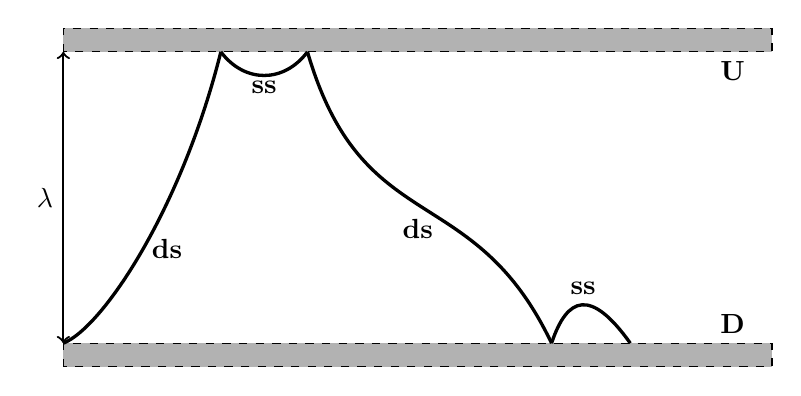
\begin{tikzpicture}
\usetikzlibrary{arrows}
\draw[fill=gray!60,dashed] (-3,0) rectangle (6,0.3);
\draw[fill=gray!60,dashed] (-3,-4) rectangle (6,-3.7);
\draw[very thick] (-3,-3.7) .. controls (-2.5,-3.5) and (-1.5,-2) .. (-1,0);
\draw[very thick] (-1,0) .. controls (-0.7,-0.4) and (-0.2,-0.4) .. (0.1,0);
\draw[very thick] (0.1,0) .. controls (0.8,-2.4) and (2.2,-1.6) .. (3.2,-3.7);
\draw[very thick] (3.2,-3.7) .. controls (3.4,-3.1) and (3.7,-3.0) .. (4.2,-3.7);
\draw (5.5,-3.7) node (d) [above] {$\mathbf{D}$};
\draw (5.5,0) node (u) [below] {$\mathbf{U}$};
\draw (-2.0,-2.5) node (ds1) [right] {$\mathbf{ds}$};
\draw (-0.45,-0.25) node (ss1) [below] {$\mathbf{ss}$};
\draw (1.5,-2) node (ds2) [below] {$\mathbf{ds}$};
\draw (3.6,-3.2) node (ss2) [above] {$\mathbf{ss}$};
%\draw [dashed,thick] (0,0.8) node (zaxis) [above] {$\mathbf{z}$}
%        |- (0.8,0) node (yaxis) [right] {$\mathbf{y}$};
\draw [<-,thick] (-3.,-3.7) -- (-3,-1.85) node (d) [left] {$\mathbf{\lambda}$};
\draw [<-,thick] (-3,0) -- (-3,-1.85);
\end{tikzpicture}
}
\end{center}
\caption{ A full scenario of electron's trajectories between parallel plates, including both double surface (ds) and single surface (ss) impacts. \cite{Non}\label{fig:ss-ds}}
\end{figure}

The basic idea of the non-stationary theory is that, as the initial velocity $u$ of emitted particles is a random variable, the solution of equation \eqref{nposition} w.r.t the time $\tau$ that particles hit the plates actually is the joint probability that an electron released at phase $\varphi_s$ impacts with the opposite wall, separated by $\lambda$, in a transit time $\tau$. As long as we know the probability density function (PDF) of the initial velocity $u$, which usually is a thermal distribution, then the joint PDF can be derived according to the rule of change of variable in probability theory. 

Following the definitions in Ref \cite{Non}, each plate will be denoted as $D$ and $U$ for the boundary condition $\xi=0$ (down) and $\xi=\lambda$ (up), respectively. Double and single surface impacts with $D-U$ or $U-D$ and $D-D$ or $U-U$ trajectories will be denoted as $ds$ and $ss$ respectively. Other definitions for the non-stationary theory are given in \cite{Non}, and listed here in Table \ref{my_table} for convenience.
\begin{table}[h]\footnotesize
{\renewcommand{\arraystretch}{1.5}
\renewcommand{\tabcolsep}{0.2cm}}
\caption{Non-stationary theory definitions.}
\centering
  \label{my_table}
  \begin{tabular}{ l  r  }
    \hline
\hline			
    Impact rate (electrons/radian) in plate $U/D$ at phase $\varphi$ & $I_{U/D}(\varphi)$ \\
    Emission rate (electrons/radian) in plate $U/D$ at phase $\varphi$ & $C_{U/D}(\varphi)$ \\
    Number of electrons at time $\varphi$ & $N(\varphi)$ \\
    Probability density that an electron starting at plate $U/D$,\\
    with starting phase $\varphi$, experiences a double/single\\
    surface impact in a transit phase $\tau$ & $G_{ds/ss,U/D}(\tau|\varphi)$\\
    secondary emission yield of an electron starting at plate $U/D$, with starting\\
    phase $\varphi$, experiences a double/single surface impact\\
    in a transit phase $\tau$ & $\delta_{ds/ss,U/D}(\tau|\varphi)$\\

    \hline 
 \hline
  \end{tabular}
 \end{table}

The electron emission rates and impact rates in each plate can be described by the joint PDF and the secondary emission yield coefficient, both of which are the function of initial velocity $u$, initial phase $\varphi_s$ and time $\tau$ at which particles hit the plates. Details of constructing the joint PDF and integrating the emission rates and impact rates can be found in Ref \cite{Non}. The number of electrons between the parallel plates at phase $\varphi$ then can be integrated as:
\begin{flalign}
N(\varphi)=&\int_0^\varphi \left(C_U(\varphi')+C_D(\varphi')-I_U(\varphi')-I_D(\varphi')\right)\mathrm{d}\varphi'\label{npdef}
\end{flalign}

We use the secondary emission yield curve of copper provided in reference \cite{Furman-Pivi} to benchmark the Furman-Pivi model and use the secondary emission yield curve of silver given in \cite{Non} to benchmark Vaughan's  secondary emission model.

The initial particles are equally generated in both plate U and plate D. The speed of emitted particles both in the theory and in the benchmark simulation follows the Maxwellian distribution \cite{Non}: 
\begin{equation}
f_u=\frac{uv^2_{\omega}}{v^2_t}\exp{\left(-\frac{u^2v^2_{\omega}}{2v^2_t}\right)}.\label{maxwellian}
\end{equation}
\subsection{Benchmark Results}
The first set of parameters we have chosen to perform benchmark is: $f=200$MHz, $V_0=1200$V, $d=30$mm. The material of the multipactor is copper and we calculate the time evolution of the particle number. The results, using  Furman and Pivi's secondary emission model matches the theoretical model very well, as can be seen from figure \ref{fig:results}.   
\begin{figure}[]
\begin{center}
\includegraphics[width=0.7\textwidth]{figures/match.pdf}
\end{center}
\caption{Time evolution of electron number predicted by theoretical model and \opal\ simulation using Furman and Pivi's secondary emission model at $f=200$MHz, $V_0=1200$V, $d=30$mm.\label{fig:results}}
\end{figure}

The time evolution of electron number under above parameters reaches some equilibrium conditions that the electron population is nether strongly increased nor decreased. The strong multiplication cases have also been observed during benchmark:
\begin{figure}[H] 
  \subfigure[]{ 
    \label{fig:multi_copper} %% label for first subfigure 
    \begin{minipage}[]{0.5\textwidth} 
      \centering 
      \includegraphics[width=3.8in]{figures/copper_multi.pdf} 
    \end{minipage}}% 
  \subfigure[]{ 
    \label{fig:multi_silver} %% label for second subfigure 
    \begin{minipage}[]{0.5\textwidth} 
      \centering 
      \includegraphics[width=3.8in]{figures/silver_multi.pdf} 
    \end{minipage}} 
%  \subfigure[]{ 
%    \label{fig:de} %% label for second subfigure 
%    \begin{minipage}[]{0.8\textwidth} 
%      \centering 
%      \includegraphics[width=1\textwidth]{models_comp.pdf} 
%    \end{minipage}} 
  \caption{(a) Time evolution of electron number at $f=200MHz$, $V_0=120V$, $d=5mm$, using Furman and Pivi's model in simulation and copper's SEY data in theory; (b) Time evolution of electron number at $f=1640MHz$, $V_0=120V$, $d=1mm$, using Vaughan's model in simulation and silver's SEY data in theory.} 
  \label{fig:mini:subfig} %% label for entire figure 
\end{figure}

The deviations of simulation results in figure \ref{fig:multi_copper} and figure \ref{fig:multi_silver} over the theoretical model predicted values are very small and will not increase as integration time increases, as is shown in figure \ref{fig:de}.

\begin{figure}[H]
\begin{center}
\includegraphics[width=0.7\textwidth]{figures/models_comp.pdf}
\end{center}
\caption{Time evolution of relative deviations of simulation results using Furman-Pivi's model and Vaughan's model over theoretical model predicted values.\label{fig:de}}
\end{figure}

The re-normalization of simulation particles approach has also been benchmarked in the way that the effective particle number per simulation particle in each time step is determined by the current of each simulation particle divided by the initial current of each simulation particle. Again, the agreements among the re-normalization of simulation particles approach, the real emission particles approach and the non-stationary theory are very good.
\begin{figure}[H] 
  \subfigure[]{ 
    \label{fig:const_multi_copper} %% label for first subfigure 
    \begin{minipage}[]{0.5\textwidth} 
      \centering 
      \includegraphics[width=3.8in]{figures/const_particle_benchmark_FurmanPivi.pdf} 
    \end{minipage}}% 
  \subfigure[]{ 
    \label{fig:const_multi_silver} %% label for second subfigure 
    \begin{minipage}[]{0.5\textwidth} 
      \centering 
      \includegraphics[width=3.8in]{figures/const_particle_benchmark.pdf} 
    \end{minipage}} 
  \caption{(a) Time evolution of electron number predicted by theoretical model and \opal\ simulation using Furman-Pivi's secondary emission model with both re-normalization of simulation particle approach and real emission particle approach at $f=200MHz$, $V_0=120V$, $d=5mm$; b) Time evolution of electron number predicted by theoretical model and \opal\ simulation using Vaughan's secondary emission model with both re-normalization of simulation particle approach and real emission particle approach at $f=1640$MHz, $V_0=120$V, $d=1$mm.} 
  \label{const_simu} %% label for entire figure 
\end{figure}
\begin{figure}[H]
\begin{center}
\includegraphics[width=0.7\textwidth]{figures/models_comp_const_part.pdf}
\end{center}
\caption{Time evolution of relative deviations of simulation results using Furman-Pivi's model and Vaughan's model with re-normalization of simulation particle approach over theoretical model predicted values. \label{fig:const_de}}
\end{figure}
\section{APPLICATIONS}
\subsection{Multipacting Study on a Cyclotron RF Cavity}
After benchmark, we can use the above newly developed tool in \opal\ to study the multipacting property of the RF cavities in real accelerator. The test case here is the RF cavity of CYCIAE-100 \cite{Zhang20084117}, a 100 MeV H- AVF cyclotron under construction at China Institute of Atomic Energy (CIAE). 

According to experiments performed by Cern for LHC project, the SEY curve of copper can vary dramatically with different surface treatments \cite{seycurve}. It will be interesting to predict the multipacting phenomena in the conditions with or without surface treatment for the under manufacturing RF cavity of CYCIAE-100. The SEY curves in figure \ref{fig:sey} are fit to the experiment data in Ref \cite{seycurve} with the equation \eqref{Vaughanall} and will be used in the simulations, as they correspond to the SEY of copper without surface treatment and the SEY of copper with the most probable surface treatment and installation condition that we will use for the cavity, i.e., the sputter cleaned surface with several days exposure to air outside the vacuum chamber, respectively.   
\begin{figure}[H]
   \centering
  \includegraphics*[width=0.7\linewidth,angle=0]{figures/diff_SEYCurve.pdf}
   \caption{The SEY curve of copper used in this multipacting study (modeled by Vaughan's formula).}
   \label{fig:sey}
\end{figure}

The RF cavities will be installed in the valley of the cyclotron magnet and therefore will be exposed under magnetic stray field of a few hundreds of Gauss (see the figure \ref{fig:valley}). This stray field is also modeled in the simulation.

%how to include figures

\begin{figure}[H]
   \centering
  \includegraphics*[width=0.7\linewidth,angle=0]{figures/Bfield_Cavity.jpg}
   \caption{The RF cavity of CYCIAE-100 cyclotron under the magnetic stray field.}
   \label{fig:valley}
\end{figure}
 The electromagnetic field used in the simulation is at the full RF power and the initial electrons will be randomly generated near the surface of the cavity where the electric field is larger than a threshold (2MV/m), as is shown in figure \ref{fig:initial}. 
\begin{figure}[H]
   \centering
  \includegraphics*[width=0.5\linewidth,angle=0]{figures/initial_field_particle.jpg}
   \caption{The electric field in the cavity and initial distribution of electrons (projection view at the symmetric plane of the cavity along the radius).}
   \label{fig:initial}
\end{figure}

Figure \ref{fig:seydiff} shows the time evolution of particle numbers. The multipacting has been observed in both with and without surface treatment cases, but the multiplication of the case without surface treatment is 5 magnitude larger than the case with surface treatment. In real case, such large magnitude difference will significantly increase the risk of surface etching and consequently cause RF breakdown. 

\begin{figure}[H]
   \centering
  \includegraphics*[width=0.7\linewidth,angle=0]{figures/diff_SEY_comparison.pdf}
   \caption{The time evolution of particle numbers in both with and without surface treatment cases, the phase lag of both cases are 0 degree.}
   \label{fig:seydiff}
\end{figure}

 We have also studied the phase dependence of multipacting phenomena at the full RF power. The SEY curve of copper with surface treatment is used for this parameter study. The parameter under evaluation is the RF phase lag from 0 degree to 180 degree with 5 degree's interval. The preliminary results show an obvious phase selection property of multipacting phenomena. Figure shows the time evolutions of electron population with different RF phase lag.

  
\section{CONCLUSIONS AND DISCUSSIONS}
Enlightened by a triangulated surface representation of geometries and an efficient particle-boundary collision test, RF components with arbitrary, closed structure, like electron gun and cyclotron resonators can be modeled in \opal\ for dark current and multipacting simulation. The carefully performed benchmark against the non-stationary multipacting theory gives us a strong confidence on using \opal\ as a prediction tool of multipacting phenomena for RF structure design.

The preliminary results for the test cases have demonstrated the capability of \opal\ on dark current and multipacting simulation. Post processing utilities, like the hot spot visualization and time evolution of particle distribution, are useful to locate the multipacting zone. 

Further multipacting simulations are planed for the CYCIAE-100 cyclotron cavity on different RF power level to better understand the multipacting behavior of the cavity during the RF conditioning process and hopefully can shorten the time consumption on the RF conditioning process. 
\section{ACKNOWLEDGMENTS}
The authors thank the Accelerator Modeling and Advanced Simulation (AMAS) group members C.\,Kraus, Dr. B. Oswald and H. Guo for many discussions regarding programming and visualization. This work was performed on the {\it felsim} cluster at the Paul Scherrer Institut.

\bibliography{mp-phys-rev-stab}

\end{document}

